\documentclass[11.5pt]{sig-alternate}
\usepackage[defaultlines=3,all]{nowidow}
\usepackage{hyperref}
\usepackage{tabularx}
\usepackage{graphicx}
\usepackage{blindtext}
\usepackage[utf8]{inputenc}
\usepackage[english]{babel}
\usepackage{lastpage}
\usepackage{comment}
\usepackage{dirtytalk}
\usepackage{xcolor}
\usepackage{hanging}
\usepackage{wrapfig}
\usepackage[backend=biber, style=apa]{biblatex}
\addbibresource{notation.bib}
\usepackage{authblk}
\usepackage{caption}
\usepackage{graphicx,subfigure}
\usepackage{authblk}
\usepackage{enumitem}
\usepackage[utf8]{inputenc}
\usepackage{cuted}
\usepackage{fancyhdr}
\pagestyle{fancy}
\usepackage{lipsum}
\usepackage{microtype}
\renewcommand{\headrulewidth}{0pt}
\renewcommand{\footrulewidth}{0pt}
\setlength\headheight{80.0pt}
\addtolength{\textheight}{-80.0pt}
\chead{%
  \ifcase\value{page}
  % empty test for page = 0
  \or 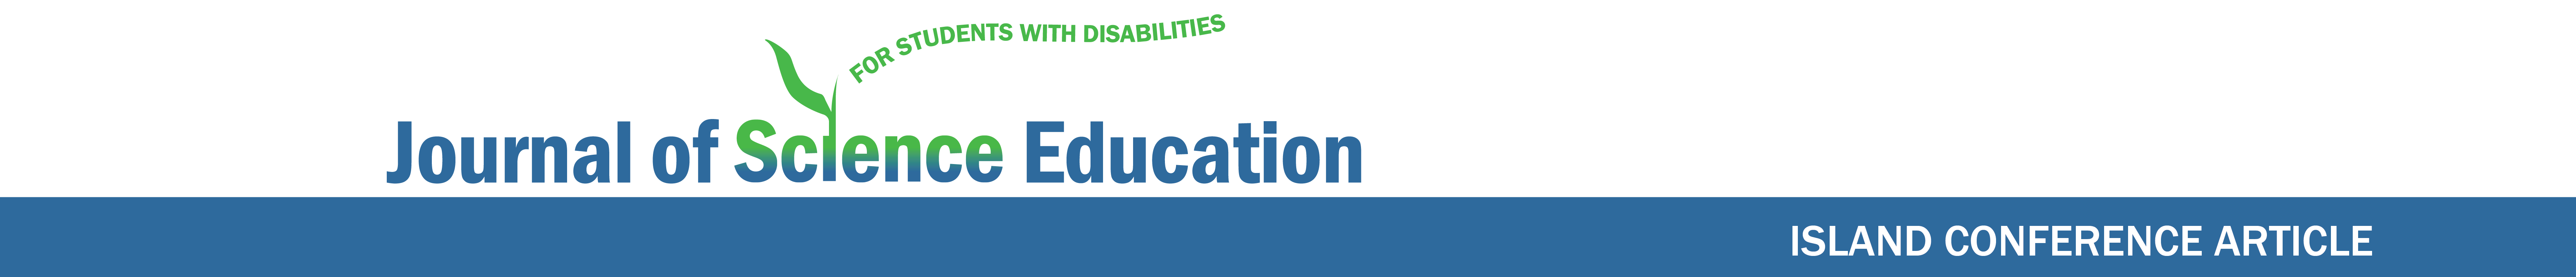
\includegraphics[width=\textwidth]{headerimage.png}% page = 1
 \or 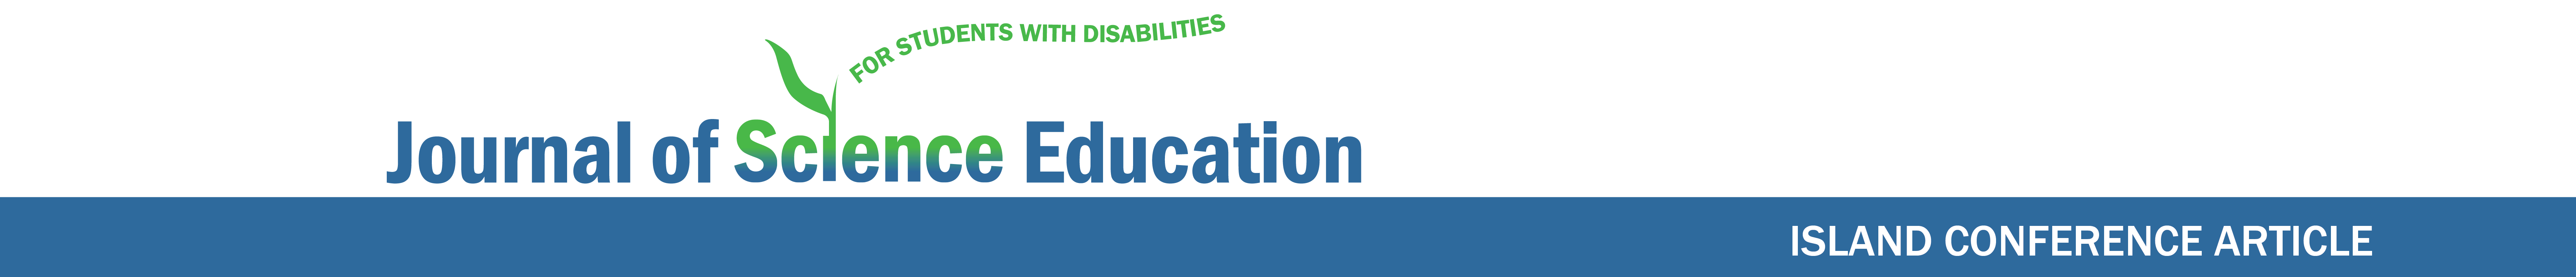
\includegraphics[width=\textwidth]{headerimage.png}% page = 2
  \or 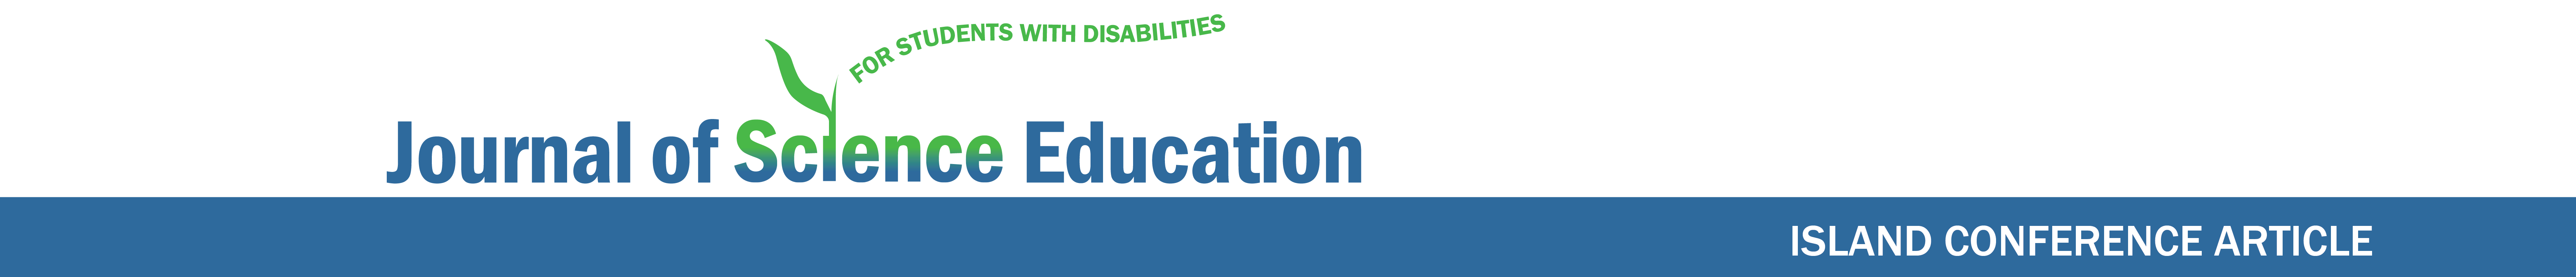
\includegraphics[width=\textwidth]{headerimage.png}% page = 3
  \or 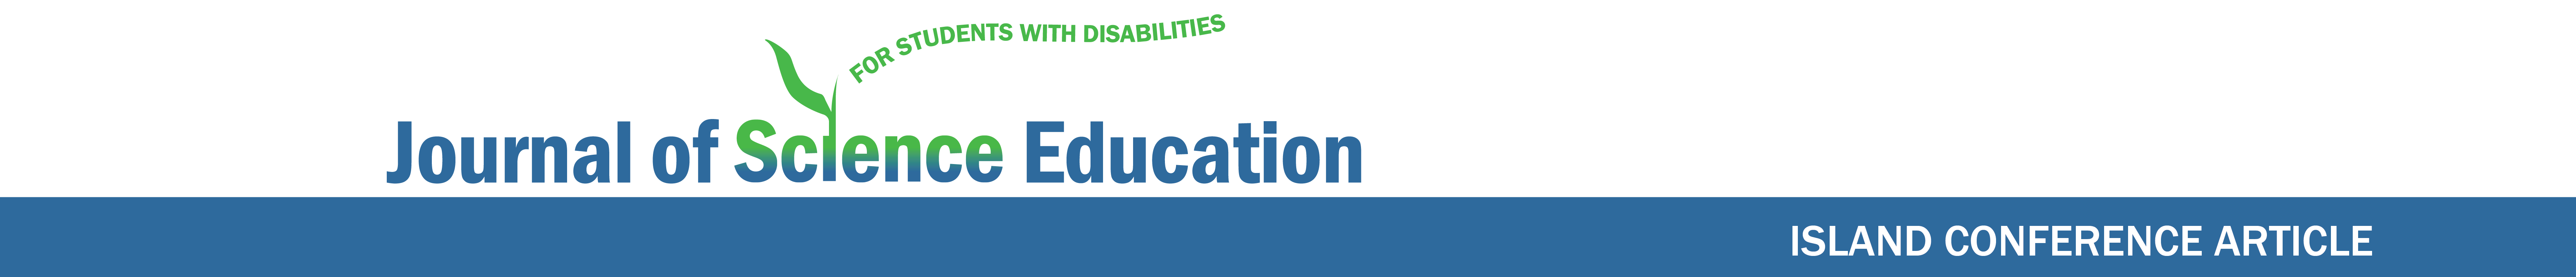
\includegraphics[width=\textwidth]{headerimage.png}% page = 4
 \or 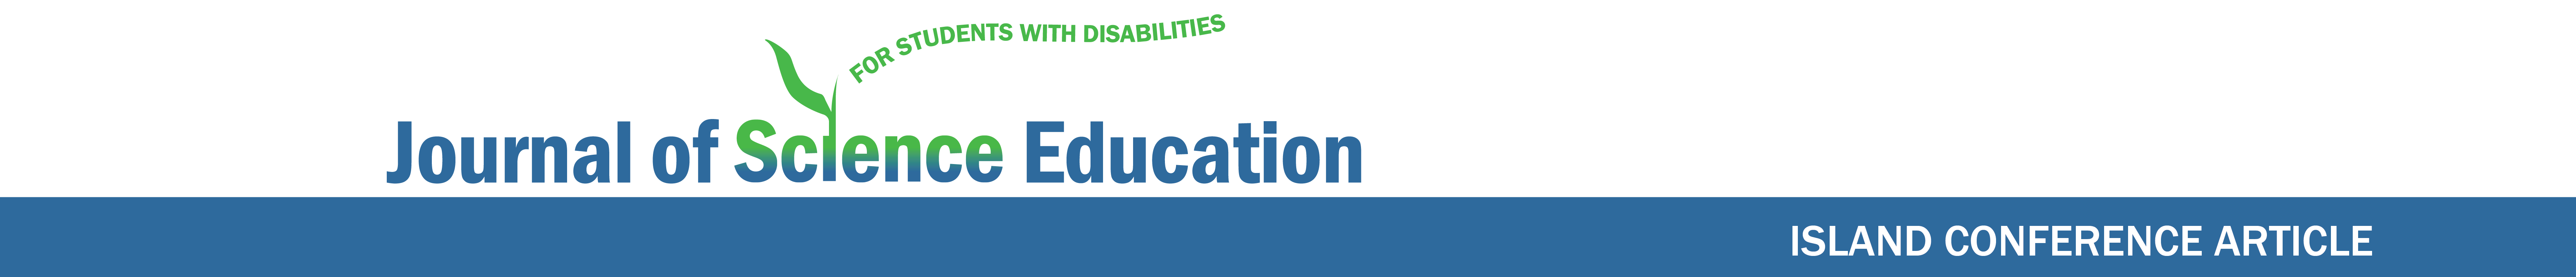
\includegraphics[width=\textwidth]{headerimage.png}% page = 5
  \else
  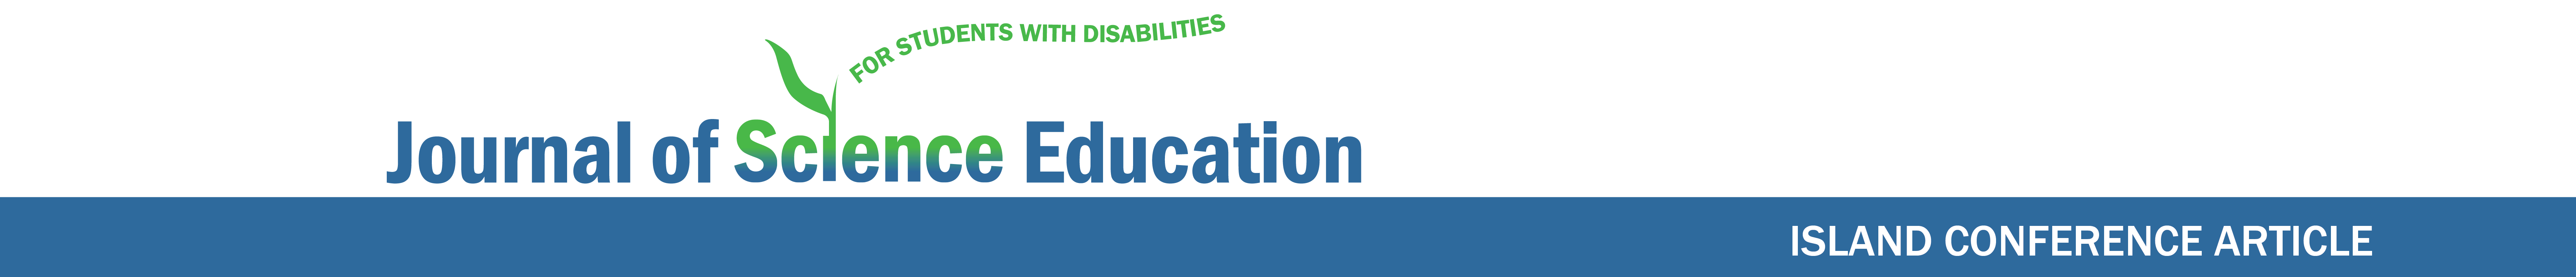
\includegraphics[width=\textwidth]{headerimage.png}
  \fi
}
% set caption and figure to italics
\captionsetup[figure]{font = it,}
\captionsetup[table]{font = it,}
%\chead{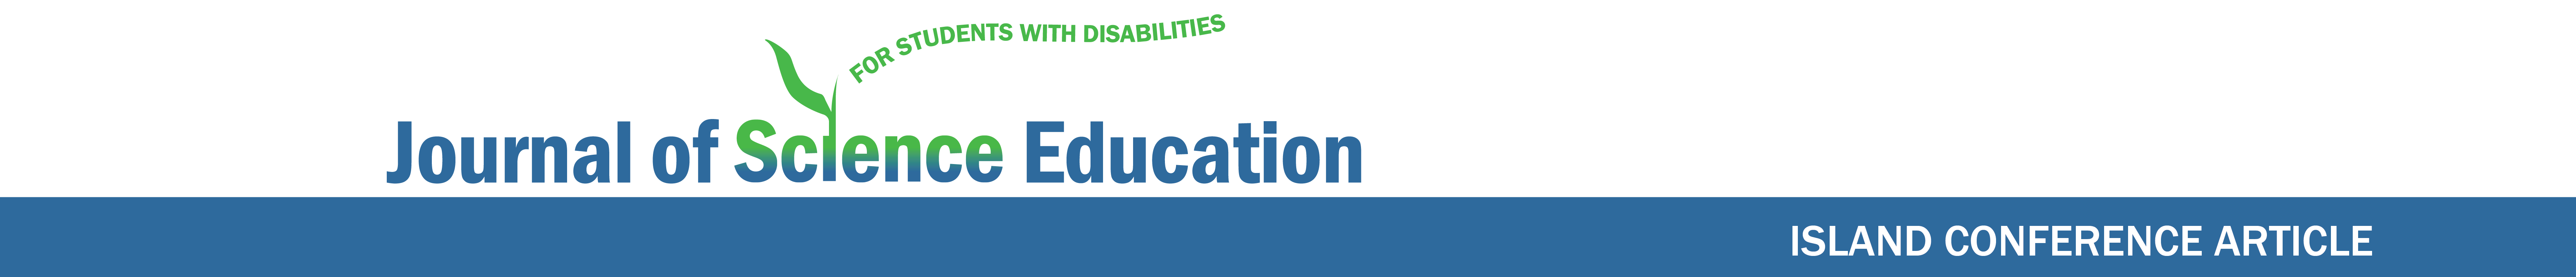
\includegraphics[width=\textwidth]{headerimage.png}}
\hypersetup{
    colorlinks=true,
    urlcolor=blue
}
 
\let\oldabstract\abstract
\let\oldendabstract\endabstract
\makeatletter
\renewenvironment{abstract}
{\renewenvironment{quotation}%
               {\list{}{\addtolength{\leftmargin}{1em} % change this value to add or remove length to the the default
                        \listparindent 1.5em%
                        \itemindent    \listparindent%
                        \rightmargin   \leftmargin%
                        \parsep        \z@ \@plus\p@}%
                \item\relax}%
               {\endlist}%
\oldabstract}
{\oldendabstract}
\makeatother

% Left align captions
\captionsetup{justification   = raggedright,
              singlelinecheck = false}


\begin{document}

\title{The PLAYground: An Online Summer Camp for Deaf and Hard of Hearing Children}

\author[1]{\large \color{blue}Emma Monson}
\author[1]{\large \color{blue}Krista Schumacher}
\author[1]{\large \color{blue}AnnMarie Thomas}

\affil[1]{University of St. Thomas, Minnesota}

\toappear{}
%% ABSTRACT
\maketitle
\begin{@twocolumnfalse} 
\begin{abstract}
\item 
 \textit {The PLAYground summer camp was developed by the Playful Learning Lab (PLL) at the University of St. Thomas, an undergraduate research group with a focus on learning through play. Through a partnership with a local school serving deaf and hard of hearing students, the PLAYground was designed to provide content to the deaf and hard of hearing community. Over the course of 8 weeks, 84 students were provided with materials that correspond with activities on the website. Each activity is accompanied with a lesson plan and video, both of which are available in English, American Sign Language, Spanish, and Arabic. Students participating in the PLAYground also had the option to meet with camp counselors via Zoom weekly to build community and create together.}
     \\
     \\
     Keywords: play, learning, deaf education, online, summer camp
\end{abstract}
\end{@twocolumnfalse}

%% AUTHOR INFORMATION

\textbf{*Corresponding Author, Emma Monson}\\
\href{mailto: mons7894@stthomas.edu }{(mons7894@stthomas.edu)} \\
\textit{Submitted January 8, 2021 }\\
\textit{Accepted February 25, 2021} \\
\textit{Published online September 16, 2021} \\
\textit{DOI:10.14448/jsesd.13.0008} \\
\pagebreak
\pagebreak

\vspace{5mm}
\section*{\vspace{140mm}}
\begin{large}
    \section*{THE PLAYGROUND: AN ONLINE SUMMER CAMP FOR DEAF AND HARD OF HEARING CHILDREN}

The PLAYground summer camp was developed by the Playful Learning Lab (PLL) at the University of St. Thomas, an undergraduate research group with a focus on learning through play. Members of the PLL come from a wide range of majors, including education, engineering, communications, and many more. Combined, this allows the lab to run a variety of projects, with many different local partners. Some of the major projects of the PLL include OK Go Sandbox, Deaf Education, Minnesota Children’s Museum, and Circus Science. Each of these require a partnership with an outside party, and the lab creates resources for these partners and educators around the world. 

The PLL has partnerships with two local schools serving deaf and hard of hearing students: Metro Deaf School in St. Paul, Minnesota, and Minnesota State Academy for the Deaf in Faribault, Minnesota. At both of these schools, the PLL hosts afterschool STEAM workshops, where students are encouraged to complete design challenges using their creativity. A main focus of these afterschool programs is to help students learn the engineering design process and embrace failure, rather than see it as having negative effects. Students are encouraged to work together to find solutions to projects, as sharing ideas can help students find new ideas and build off of each other. Previous research on this program with Metro Deaf School has shown that exposure to STEM content can increase student’s confidence, interest, and progress in seeing themselves as capable of one day becoming an engineer (Kasper et al., 2016). Using this research, our intent was to continue offering hands-on experiences that students could participate in with hopes that they would have a positive mindset when faced with a STEM challenge. 

Before the COVID-19 pandemic began, the PLL hosted in-person afterschool STEM/STEAM workshops at both Deaf schools. This involved two or three members of the PLL traveling to the schools and bringing along the necessary materials for a variety of pre-planned STEM activities including parachutes, slime/oobleck, and the egg drop challenge. For each activity or challenge, the students were given instructions and various constraints for what they were building. Instruction came from the PLL members, with the assistance of an interpreter. An example of one of our workshops was the parachute challenge, which was an especially engaging activity for the students. After they were given the basic premise of what a parachute is and a few hints for creating their parachute, they had time to construct, test, and potentially reconstruct their creation. We saw high levels of participation as students kept running upstairs to test their parachutes and then create a new iteration to make it fall more slowly to the ground. 

Due to COVID-19, the PLL was unable to finish the year with in-person STEAM workshops. After a few months of not being with the students in person, the PLL worked on finding ways to connect with the students virtually. This is what prompted the idea of creating an online summer camp. This began as a simple idea of giving students at Metro Deaf School materials and accompanying lesson plans, with optional weekly Zoom meet-ups to complete activities. This soon evolved into a camp that would be offered to locals in the deaf community (especially those who attend Metro Deaf School and Minnesota State Academy for the Deaf). Members of the PLL then began to determine what we wanted to include in our camp. We wanted the camp to be accessible to as many students and families as possible, so we assembled teams within the PLL and Metro Deaf School to create content in English, Spanish, Arabic, and American Sign Language.

Over the course of eight weeks, 84 students were provided with free materials that correspond with activities on the PLAYground website (Figure 1). These materials were provided in a box, with all necessary items for that week’s activities (Figure 2). Starting with week one, students were given all the specific materials for those lessons, along with a scissors, glue stick, tape, and other materials that may be needed throughout the course of the eight week camp. This was done to ensure that all students had the same items, whether or not they had previously had them at home. Every week, students received a box of materials that they would use throughout that whole week. Materials were hand-delivered by members of the PLL. This part of the summer camp process was very important to the PLL. It gave our team a chance to see the students (through doors and windows due to the pandemic) and see their excitement of receiving a new box for the week. Although we could not interact with students in person, getting to see them for a minute or two was a great way to connect with them off-screen. 

\begin{figure}[h]
    \centering
    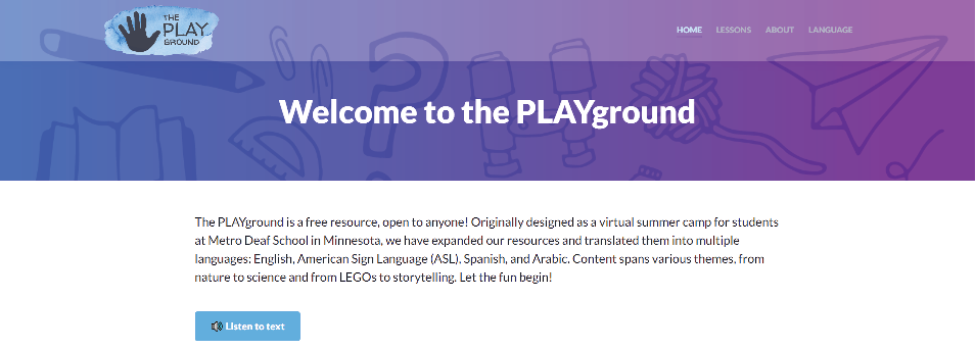
\includegraphics[width=8cm]{figure 1.png}
    \caption{The homepage of the PLAYground website.}
\end{figure}

\begin{figure}[h]
    \centering
    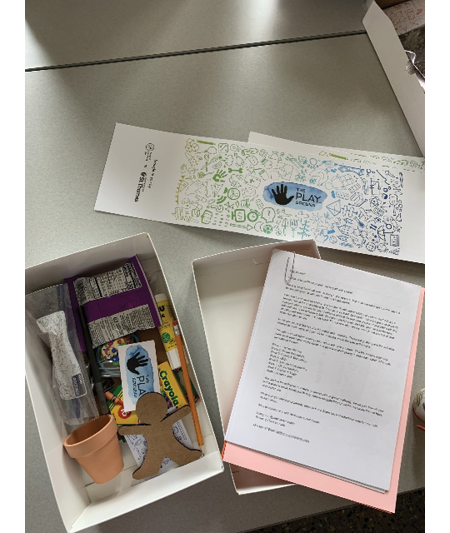
\includegraphics[width=8cm]{figure 2.png}
    \caption{A box for one week, containing: a letter for the parents, activity materials, and snacks}
\end{figure}

Accessibility is a major focus and concern of the PLL, especially when COVID-19 hit. It was important to give all students the same materials, so as not to assume that they would have any of the necessary items, as well as make sure that they all had access to the same materials. Something as simple as a pair of scissors gave each student the opportunity to participate and increased the camp’s accessibility. The PLL believes that accessibility in physical resources and language-based resources was vital to the success of the summer camp. We did not want language or access to physical items to be a barrier that prevented participants from engaging with the content or their peers and camp counselors. We also hope that providing written and video lessons in various languages increases the audience that can interact with the PLAYground’s online content, even if they were not part of the summer camp program. At the conclusion of the summer camp, we hoped that families and educators around the world would use the resources available on the website to encourage playful learning in their children or students. 

Each activity is accompanied by a lesson plan and video, each available in English, American Sign Language, Spanish, and Arabic (Figure 3). Because accessibility was one of the main focuses for the PLAYground, we wanted all students and their families to have full access to all of the provided resources. The PLL members set up teams of Spanish and Arabic translators, and we brought in assistance from teachers and staff at Metro Deaf School for our American Sign Language videos. 

\begin{figure}[h]
    \centering
    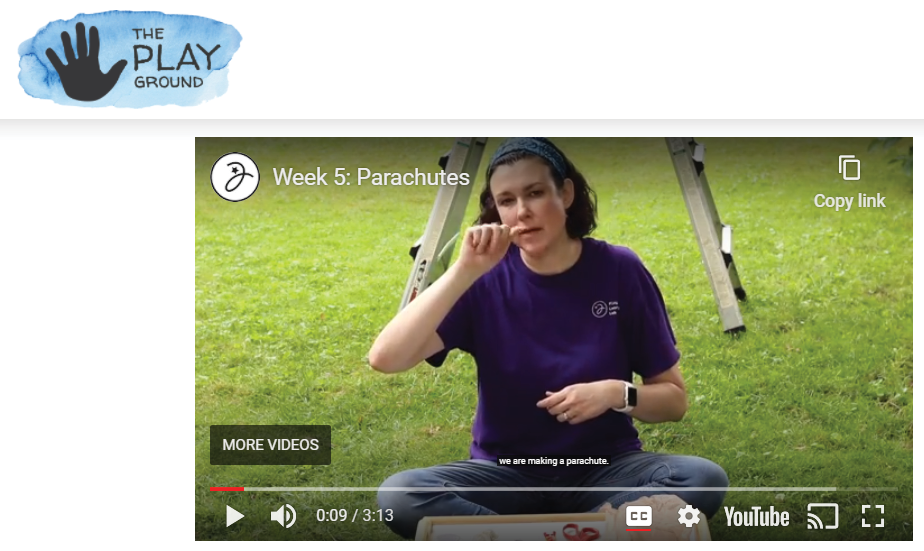
\includegraphics[width=8cm]{figure 3.png}
    \caption{An example lesson video shown in American Sign Language (ASL) with English closed captioning.}
\end{figure}

Students participating in the PLAYground also had the option to meet with camp counselors weekly via Zoom to build community and create together. Not all participants chose to attend these Zoom meetings. Those who did join the meetings were encouraged to present and share what they had already created during the video call. This gave them a chance to show off their work and get positive feedback from both counselors and peers. The Zoom meet-ups also gave the students a chance to ask for help or clarification on the projects. Oftentimes, students and counselors would work on a project together, so they could show their final work at the end of the meeting. It was important for students to connect with other students, as well as counselors, to give them social time with people outside of their family. Although meeting on Zoom is not the same as meeting in person, students were able to share stories and ideas, much like how they would have if the camp was held in person. Developing these relationships allowed students to grow their social-emotional skills; they might not have had the experiences and opportunities to do so due to the shift to distance learning amidst the pandemic, as many schools offered asynchronous lessons. 

Furthermore, in alignment with our mission of accessibility, every Zoom meeting was hosted by at least two counselors from the PLL, as well as an interpreter. This allowed us to communicate with all of our deaf and hard of hearing students. It was important to have an interpreter at all meetings to ensure that the students were not missing out on information or time with their peers. Another important aspect of these Zoom meetings was keeping the group numbers small to ensure that all students were able to see each other and the interpreter. This showed each student that they were wanted at that meeting and the time spent with them was important to their counselors and peers. It also provided an opportunity for all student voices to be heard, showing that each individual is valuable. Groupings were determined by grade levels, such as Kindergarten-2nd grade, 3rd grade-5th grade, and 6th grade-8th grade.

Zoom also offers the options of pinning or spotlighting someone on a video call. This meant that participants who needed an interpreter could pin the interpreter, so they always could see someone speaking in American Sign Language on their screen. Participants also had access to the chat to communicate in side conversations with their peers or camp counselors, or to ask for help if necessary. We learned that we can increase the group size by spotlighting who is speaking and interpreting, so that all participants can see the person speaking even in a larger group. This helped to ensure that all participants were able to have a visual of the interpreter, as well as their counselor, who was showing them the project or giving instructions. During the Zoom calls, the counselors led the group in a variety of ways. On some calls, the participants had questions about specific activities and would have time to get these questions answered. On others, the group would choose an activity and do it together. On most calls, participants had time to show the projects they had completed and see what their peers had been working on throughout the week. 

A major benefit of the PLAYground was that the PLL was able to make activities public by creating a website to showcase many lessons that have been/are used throughout the year at different events. Similar to the PLAYground, the Code + Chords program has been used by the PLL in a variety of settings and is now on the website with an accompanying lesson plan for anyone to access. This goes for many lessons and projects that the PLL teaches and creates. The PLAYground website can be used by both informal and formal educators, and will hopefully be used by teachers as activities in their classrooms. 

The PLL received a large amount of feedback from participants, parents, interpreters, and other community members that were involved with the summer camp. Overall, parents seemed enthusiastic to have some sort of peer connection and hands-on activities for their child. Students who participated often enjoyed sharing time and experiences with their peers and meeting new members of the deaf and hard of hearing community across the state. Metro Deaf School teachers who helped create ASL content and joined Zoom meetings with the students were happy to stay involved with the students through the summer and offer support for them. Due to the overwhelming amount of positive feedback and generous support of the PLL’s donors, we have been able to continue the use of the PLAYground website content with other underrepresented groups around the Twin Cities through the duration of the COVID-19 pandemic. The website is available and free for anyone to access at \url{www.playgroundcamp.org}. Please feel free to access it and share it far and wide! 

Looking toward the future, we plan to continue providing materials and resources that can be used by both students and teachers at Metro Deaf School and Minnesota State Academy for the Deaf, as well as posting them online for anyone to access for free. While still in the pandemic, this involves packing materials for specific activities and delivering them to the Deaf schools, where they can be distributed to the students. In addition, the PLL is partnering with teachers at Metro Deaf School to help create lessons or resources that will help them to run their classrooms. For example, we are working with the teacher for the DeafBlind who is working with LEGO Braille Bricks to help the students with their language learning. We are also 3D printing materials, such as a map of Minnesota or the United States, as a resource for these students to learn more about geography in a tactile way. After the pandemic is over, there will be many opportunities for us to continue the work we have been doing for the past 10 months, as well as hope for returning to our in-person workshops. 

\section*{ACKNOWLEDGEMENTS}
The Playful Learning Lab would like to thank the LEGO Foundation, the No Starch Press Foundation, and Cognizant for supporting this work.
\end{large}
\include{} 
\section*{REFERENCES}\par 

\leftskip 0.25in
\parindent -0.25in 

Kasper, B., Haugh, A., Kasper, N., Gunderson, B. D., Thomas, A. P., \& Besser, D. (2016, June). \textit{Design, Implementation, and Assessment of an After-School Engineering Program for Deaf Students}. Paper presented at 2016 ASEE Annual Conference \& Exposition, New Orleans, Louisiana. 10.18260/p.26688
\end{document}